\section{Objective Caml}

Objective Caml or, in short, OCaml~\cite{OcamlDef, Remy} is a high-level programming language which 
has been developed, distributed and supported by INRIA (Institut National de Recherche en 
Informatique et en Automatique, France) since 1985. As a member of ML family this language 
provides a number of well-known statically typed functional programming features such as
first-class high-order functions, parametric polymorphism and type inference. In addition
OCaml consistently incorporates object-oriented traits --- objects and classes with 
structural subtyping, rich module system with first-class modules and \emph{functors} (that is, 
modules parameterized by other modules) which makes it a full-fledged multiparadigm programming
language. In addition OCaml is equipped with a syntax extension tools --- 
CamlP4\footnote{http://brion.inria.fr/gallium/index.php/Camlp4}/CamlP5\footnote{http://pauillac.inria.fr/\textasciitilde ddr/camlp5/} --- which allow to extend the host language with domain-specific constructs. 

We argue that in its present state OCaml is already rich enough to be directly used as an 
implementation formalism for all the tasks listed for the tool challenge. Apart from parsing and 
pretty-printing which can easily be handled in a standard way using parser- and printer combinators 
the other tasks are rather simple transformations of abstract syntax trees. The main consideration
for the OCaml implementation was to utilize \emph{type-driven transformers} to express all these
transformations. As we deal with the extending family of languages we have to resort to extensible
data structures and, respectively, extensible type-driven transformers. As we will see in the next 
section, all these notions can nicely be implemented in the pure OCaml. 

\begin{figure}
\begin{center}
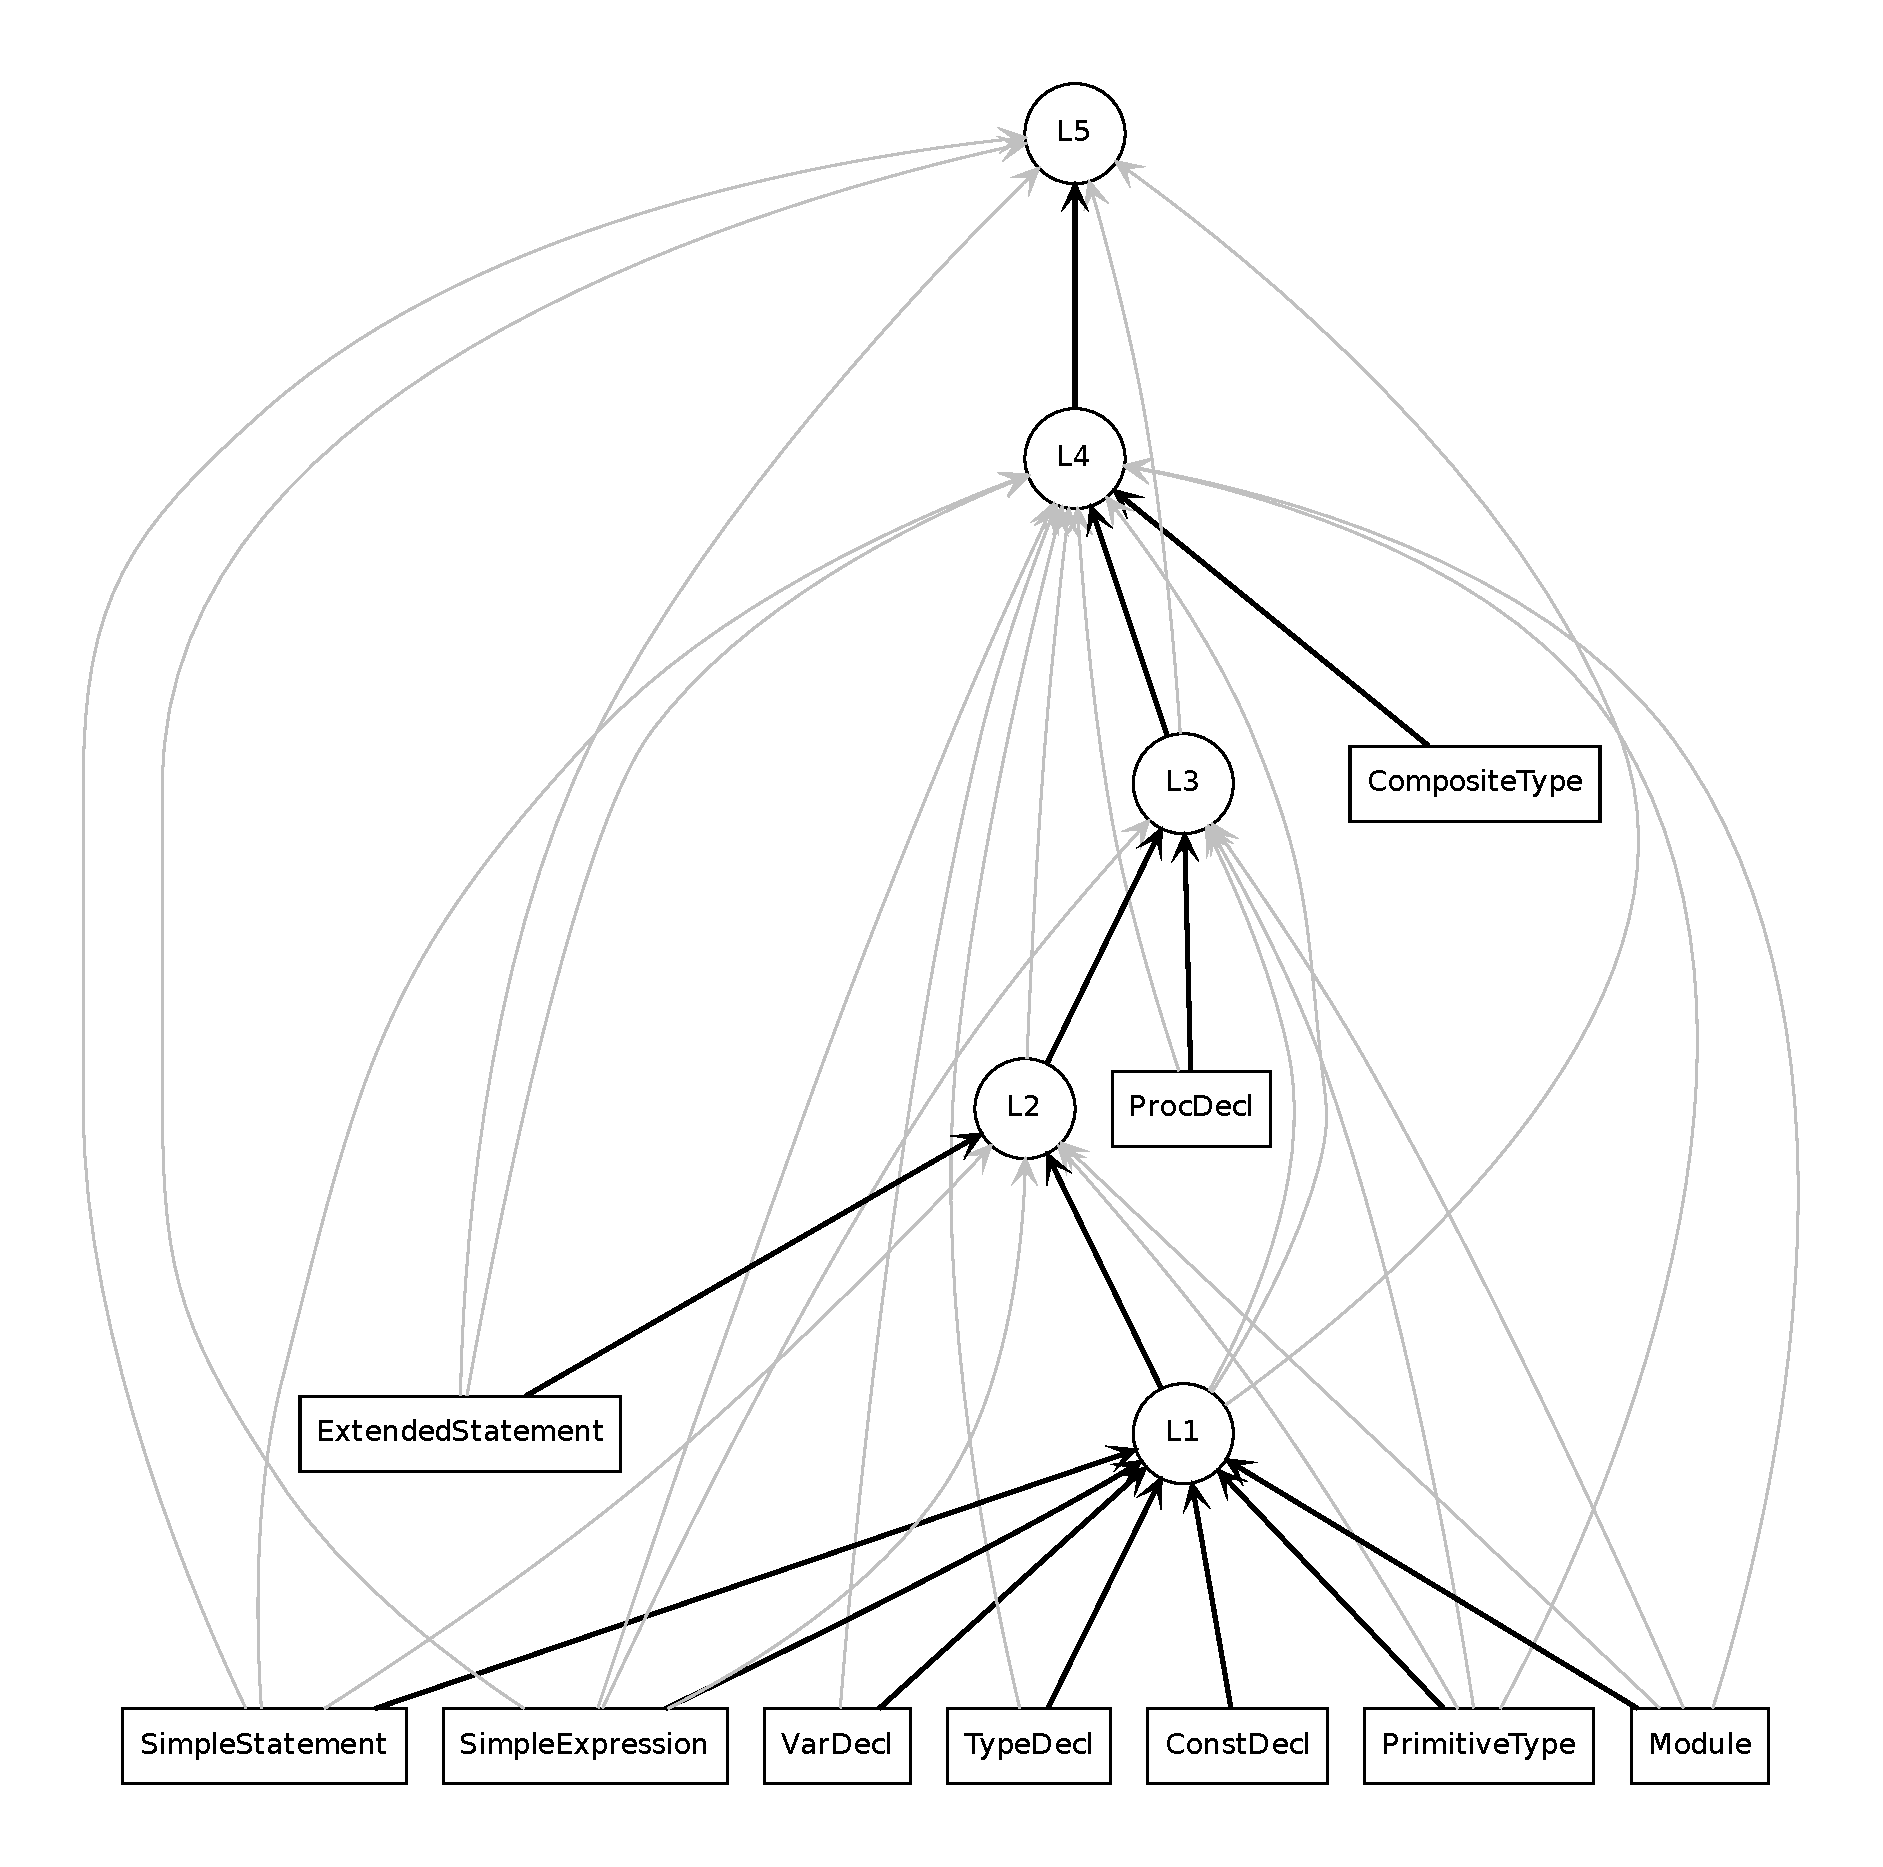
\includegraphics[height=13cm, width=14cm]{ocaml/depend.pdf}
\end{center}
\caption{OCaml Implementation Module Dependencies}
\label{ocamlmoddep}
\end{figure}

The module-wise structure of OCaml implementation is shown on Figure~\ref{ocamlmoddep}. This diagram
was converted from the actual \verb|Makefile| dependency include; some auxiliary utility modules were
omitted. Square-shaped nodes designate language components while circle-shaped stand for the 
language toplevels. Black edges emphasize a transitive reduction of module dependency relation which corresponds 
to the inter-language dependency. Each language component provides the parametrized solutions for all
tasks of the challenge for the certain syntactic category. Most of them are expressed in terms of
type-driven transformers. The parametrization allows to reuse the same functionality in a various
concrete contexts --- for example, module \verb|VarDecl| implements \emph{generic} variable declaration
construct parametrized by a type representation; this implementation provides parser, pretty-printer, name resolver,
typechecker etc., each of which are in turn parametrized by the respective functionality for type representation.
As a result the same separately compiled code is used to implement variable declarations in languages
L1-L3 (where only base types are allowed) as well as in L4-L5 (where composite types are added). This approach
allows to combine language implementations from precompiled reusable components as long as we deal with the extending
family of languages. For example, the implementation of L2 was build ``on top'' of L1 by reusing existing modules 
including L1 toplevel.


\subsection{Type-driven Transformers}

In this section we describe type-driven transformers of a certain kind which are 
massively used in OCaml implementation. Namely, all the tasks excluding parsing
are expressed using solely the transformers of this kind. ``Type-driven'' means that
the semantics of transformers is completely determined by the transforming type; 
so all transformers can be constructed mechanically from the type definitions.
The converse is also true --- the type-driven transformer unambigiously defines
some type. We heavily utilize this property --- actually there is not a single 
type definition in the implementation: all types are introduced implicitly 
and inferred from the transformation functions. Another property of transformers
is their extensibility: each transformer operates on a data of a partially-defined, 
or \emph{open}, type. Thus transformers for some types can be combined by a certain primitive
to provide a transformer for the union type which still remains open and so can be
combined later on. As a result we can construct a highly modular structure of
transformers each of which implements some task on a certain trait of some general
data structure. 

To implement this kind of approach a certain support from a host language type 
system is needed. OCaml provides such a support in particular by mean of 
\emph{polymorphic variant} types~\cite{PV}. In short, polymorphic variant types allow to 
share the same constructor between the different variant types with possibly different 
types and numbers of arguments. Polymorphic variant type need not (but can) be explicitly
declared. Another feature of polymorphic variant types is that they can be open --- in each
context only some of their constructors may be known. Polymorphic variants in OCaml 
can be used to express the solution for the \emph{expression problem}~\cite{Exproblem, PVReuse} --- 
that is, the problem of modular and type-safe implementation of extending data structure 
processing. 

We illustrate the construct of type-driven extensible transformers by the canonical
example --- expression evaluator. The idea is to implement evaluator as a
collection of functions each of which evaluates only the limited subset of expression's
nodes and then to combine them to construct the evaluator of the whole expression.

First, consider the function which transforms expression nodes corresponding to some binary 
operators --- say addition and subtraction\footnote{Polymorphic variant type constructors are 
lexically distinguished from the regular ones by the backquote as their first character.}:

\begin{lstlisting}[language=ocaml]
let rec evalAddSub ext expr =
  let self = evalAddSub ext in
  match expr with
  | `Add (x, y) -> self x + self y
  | `Sub (x, y) -> self x - self y
  | z -> ext self z
\end{lstlisting}

Here \lstinline{ext} stands for the extension function --- that is, the function which
transforms the rest of polymorphic variant type's constructors besides those transformed 
by \lstinline{evalAddSub}. Note that since we want to transform potentially recursive 
structures we have to provide extension function with it's own extension function which 
should be able to transform the all nodes of expression, including \lstinline{`Add} and
\lstinline{`Sub}. This extension function (``\lstinline{self}'') is acquired by partial
application \lstinline{evalAddSub} to \lstinline{ext}. Note that we just provided some 
transformer for the \emph{incomplete}, or \emph{open}, type since actually no (final) 
expression can be constructed using only \lstinline{`Add} and \lstinline{`Sub}. 

Now we provide similar extensible function for evaluating identifiers in some state 
\lstinline{s}:

\begin{lstlisting}[language=ocaml]
let rec evalIdent s ext expr =
  let self = evalIdent s ext in
  match expr with
  | `Ident n -> s n
  | z -> ext self z
\end{lstlisting}

Note that the semantics of these functions is almost completely type-driven; despite
we do not have any type declaration here we actually think in terms of types, not
in terms of implementation details. The only concrete implementation-dependent feature
is the essense of constructor-specific transformation; we'll get rid of this specificity 
later. Note also that these functions are completely independent of each other; thus, they 
can be implemented in a different compilation units or provided at arbitrary moments of 
program execution; this difference distingushes the approach under considerations from that 
described in~\cite{PVReuse}.

It is easy to see that certain combination (namely, type sum, or union) of open types 
implicitly defined by \lstinline{evalIdent} and \lstinline{evalAddSub} provides some meaningful
type for expression trees made of identifiers, additions and subtractions. It is desirable to
obtain the transformer for this sum type directly from the transformers of its summands without
tedious repeating boilerplate per-constructor processing. Of course this is possible.
Now we introduce the combinator which plays role of type sum:

\begin{lstlisting}[language=ocaml]
let (++) left right = fun ext s -> 
  left (fun self -> right (fun _ -> ext self)) s
\end{lstlisting}

This combinator takes extensible transformers for some open types and provides extensible transformer 
for the type of their sum. This is trivially achieved by providing appropriate extensions for each ``summands''.
For example,

\begin{lstlisting}[language=ocaml]
let evalAddSubIdent s = evalIdent s ++ evalAddSub
\end{lstlisting}

is (an extensible) function which evaluates expressions with nodes \lstinline{`Add}, \lstinline{`Sub} and
\lstinline{`Ident}. The extensibility means that we always can append some functionality expressed as
type-driven transformer to already existing functions. For example, if we want to add a new expression
node --- say, multiplication --- we always can provide a transformer for just this node and then combine 
it with the existing transformer for the others:

\begin{lstlisting}[language=ocaml]
let rec evalMul ext expr =
  let self = evalMul ext in
  match expr with
  | `Mul (x, y) -> self x * self y
  | z -> ext self z

let evalAddSubIdentMul s = evalAddSubIndent s ++ evalMul
\end{lstlisting}

et cetera. In context of the tool challenge the extensibility of transformers was used a number of times.
For example, L4 extends L1 at the expression level by adding field and array access, L2 extends L1 at the 
statement level by adding \lstinline{FOR}- and \lstinline{CASE} constructs, L3 extends L2 at the statement 
level by adding procedure invocation etc. Moreover since all partial transformers are independent on
each other it is possible to combine them in an arbitrary manner --- for example it is possible to
extend expressions with procedure invocations or combine statements and expressions into the joint type with
no modifications (or even recompilation) of their counterparts.

When we need to actually apply these transformers to a data structure we have to provide
some sort of ``ultimate'' extension function; it is easy to see that this function is just
an application; in the following snippet

\begin{lstlisting}[language=ocaml]
let apply f x = f x

let x = 
  evalAddSubIdent 
     (function "a" -> 1 | "b" -> 2 | "c" -> 3 | "d" -> 4)
     apply 
     (`Add (
        `Sub (`Ident "a", 
              `Mul (`Ident "b", `Ident "c")
        ), 
        `Ident "d"
      )
     )
\end{lstlisting}

the name \lstinline{x} would be bound to \lstinline{-1}.

In the previous examples we considered some concrete transformers --- evaluators. This means
that we need a separate transformer for the each task (say, name resolver or typechecker).
However a simple generalization would let us abstract this specificity away. Namely, 
we preserve the overall control flow of the transformers but parameterize the
actions carried out for each constructor. The generalized version of the first 
transformer is presented below:

\begin{lstlisting}[language=ocaml]
let rec gmapAddSub t ext expr =
  let self = gmapAddSub t ext in
  match expr with
  | `Add (x, y) -> t#add expr (self x) (self y)
  | `Sub (x, y) -> t#sub expr (self x) (self y)
  | z -> ext self z
\end{lstlisting}

Here \lstinline{t} stands for the constructor-wise transformer encoded
as an \emph{object} with methods ``\lstinline{add}'' and ``\lstinline{sub}''\footnote{Punctuator ``\lstinline{#}'' 
in OCaml stands for object method invocation.}.
Each method takes the results of the same transformation applied to the
direct counterparts of matched value and that value itself as arguments
and returns the result of the transformation. Now the evaluation function
can be expressed as

\begin{lstlisting}[language=ocaml]
let evalAddSub ext expr = 
  gmapAddSub (object
                method add _ x y = x + y
                method sub _ x y = x - y
              end) ext expr
\end{lstlisting}

The type system of OCaml allows objects to be implicitly typed: there is 
no need to declare object types ``in advance''. Another feature of object
types is that they can be polymorphic. This means that the definition of
\lstinline{gmapAddSub} does not introduce any artificial type restrictions
on a set of encoded transformations. For example, the copy transformation
can be expressed using the same function but different object (of different but
``compatible'' type):

\begin{lstlisting}[language=ocaml]
let copyAddSub ext expr =
  gmapAddSub (object
               method add _ x y = `Add (x, y)
               method sub _ x y = `Sub (x, y)
             end) ext expr
\end{lstlisting}

Since each concrete transformation can be expressed as a partial application of
some generic \lstinline{gmap...} function to an object-encoded per-constructor
transformation the implementation of the typ-sum combinator can be left completely 
unchanged. For example, the expression evaluator for partially defined expression
of addition, subtraction and identifiers can be implemented as

\begin{lstlisting}[language=ocaml]
let evalAddSubIdent s = 
  gmapAddSub (object
                method add _ x y = x + y
                method sub _ x y = x - y
              end) ++
  gmapIdent (object method ident _ n = s n end)
\end{lstlisting}

In this approach we can easily construct transformations via combining and
extending the predefined set of object-encoded per-type transformers; in 
particular the following transformer generator was extensively used in the course
of the implementation (as always we show the version for \lstinline{`Add}-\lstinline{`Sub}
type):

\begin{lstlisting}
let mapT f = object
               method add e x y = f e (`Add (x, y))
               method sub e x y = f e (`Sub (x, y))
             end
\end{lstlisting}

The final generalization consists of ``lifting'' the transformation functions
over some monad~\cite{Monads}. Since the only way in OCaml to parametrize over a
type constructor is to use functors we encode monads with the following \emph{module type}:

\begin{lstlisting}[language=ocaml]
module type S = 
  sig
    type 'a t
    val return : 'a -> 'a t
    val (>>=)  : 'a t -> ('a -> 'b t) -> 'b t
    val (>=)   : 'a t -> ('a -> 'b) -> 'b t
    val list   : 'a t list -> 'a list t
    val tuple  : ('a t * 'b t) -> ('a * 'b) t 
  end
\end{lstlisting}

The first three functions are conventional monadic operators while \lstinline{list} and
\lstinline{tuple} are just a supplementary shortcuts. We illustrate the monadic version of 
type-driven transformer by presenting the concrete implementation for simple expressions:

\begin{lstlisting}[language=ocaml]
module Mapper (M : Monad.S) =
  struct
    open M
    let rec gmap t ext expr = 
      let self = gmap t ext in
      match expr with
      | `Binop (op, x, y) -> tuple (self x, self y) >>= 
                             (fun (x, y) -> t#binop expr op x y)
      | `Unop  (op, x)    -> self x >>= (fun x -> t#unop expr op x)
      | `Const  x         -> t#const expr x
      |  x                -> ext self x 
  end
\end{lstlisting}

Lifing over a monad allows to express some additional features of transformations
such as error processing etc.

For the implementation of Oberon-0 we used three monads --- a variant of exception monad 
called \lstinline{Checked}, identity monad \lstinline{Id} and list monad \lstinline{List}. 
For the first two monads we provided a specialized transformation function \lstinline{cmap}
and \lstinline{imap} for each of open types used in the implementation:

\begin{lstlisting}[language=ocaml]
let cmap t ext expr =
  let module M = Mapper (Monad.Checked) in
  M.gmap t ext expr

let imap t ext expr =
  let module M = Mapper (Monad.Id) in
  M.gmap t ext expr
\end{lstlisting}

\subsection{Scanning, parsing and pretty-printing}

For scanning, parsing and pretty-printing we use the parser- and printer-combinator
library called Ostap\footnote{http://caml.inria.fr/cgi-bin/hump.en.cgi?contrib=513}. 

Ostap comprises of the set of regular monadic parser-combinators~\cite{MonadicParserCombinators} 
and a syntax extension for OCaml which allows to bind syntax definitions in
EBNF directly into compiler sources thus avoiding parser generation phase. The syntax
extension in turn is implemented using CamlP4/CamlP5 syntax extension 
tool. 

As example consider the parser definition for simple statements of L1:

\begin{lstlisting}[language=ocaml]
ostap (
  parse[ref][expr][stmt]: 
    assignment[ref][expr] 
  | ifStatement[expr][stmt] 
  | whileStatement[expr][stmt];
  assignment[ref][expr]: dst:ref ":=" src:expr {`Assign (dst, src)};
  ifStatement[expr][stmt]: 
    key["IF"] cond:expr 
       key["THEN"] thenPart:oseq[stmt]
       branches:(-key["ELSIF"] expr -key["THEN"] oseq[stmt])*
       elsePart:(-key["ELSE"] oseq[stmt])?
    key["END"] {
    `If ((cond, thenPart)::branches, listify elsePart)
  };
  whileStatement[expr][stmt]: 
    key["WHILE"] cond:expr key["DO"] stmts:oseq[stmt] key["END"] {
    `While (cond, stmts)
  }
)
\end{lstlisting}

The parser is implemented in a high-order form --- it takes as arguments a parsers
for references, expressions and statements as well. The structure of rules
repeats that of regular EBNF. We use here some predefined combinators --- \lstinline{key} 
and \lstinline{oseq} --- which are defined in a separate module. \lstinline{key} recognizes
its string argument making sure that the next symbol is a word delimiter while \lstinline{oseq}
parses a possibly empty semicolon-delimited items specified by its argument. Note that 
parameterization by statement parser \lstinline{stmt} makes the whole parser \emph{open} ---
it parses wider language than merely assing-if-while with assign-if-whiles as substatements.

The definition of parser becomes closed at the client level; for example, L1-statements
parsed with the following parser:

\begin{lstlisting}[language=ocaml]
statement: !(SimpleStatement.parse)[reference][expression][statement];
\end{lstlisting}

Here \lstinline{!(...)} used to bind arbitrary OCaml expression into EBNF rule (we use it
to call parser \lstinline{parse} from module \lstinline{SimpleStatement}), \lstinline{reference} and
\lstinline{expression} designate the parsers for L1 references and expressions respectively.

Similarly, we can easily combine different parameterized parsers to obtain parsers for more
complex constructs. For example, extended statements of L2 are parsed with the following
definition:

\begin{lstlisting}[language=ocaml]
statement[ref][cexpr][expr][stmt]: 
  !(SimpleStatement.parse)[ref][expr][stmt]
| !(ExtendedStatement.parse)[ref][cexpr][expr][stmt];
stmt: statement[reference][expression][expression][stmt];
\end{lstlisting}

Here we combine parser for simple statements with parser for extended statements (``CASE'' and ``FOR'')
into the one. Note the lack of semantic actions --- there are completely defined in corresponding
parsers. Note also that the types of syntax trees, provided by these two combined parsers are completely 
independent on each other. At the top level these types are combined by the compiler; this implementation 
is completely type-safe.

Besides parser-combinators Ostap contains a set of pretty-printer combinators, which are
in fact merely wrappers for the standard pretty-printing module \lstinline{Format}. To
convert the original AST into printing functions using these combinators we again
use type-driven transformers; for example, the expression pretty-printer looks like
the following:

\begin{lstlisting}[language=ocaml]
let gprint ps ext expr =
  let b x = hovboxed (listBySpaceBreak x) in
  let op (s, p) = string s, p in
  let w p' (x, p) = if p' < p then rboxed x else x in 
  imap  
    (object 
       method binop _ o x y = 
         let s, p = op (ps#binop o) in b [w p x; s; w p y], p
       method unop  _ o x   = 
         let s, p = op (ps#unop o) in b [s; w p x], p
       method const _   x   = ps#const x
     end
    )
    ext
    expr
\end{lstlisting}

Note that apart from extensibility this pretty-printer is generalized in yet another 
dimension --- namely, it is abstracted away from the concrete syntax. The \emph{ps}
parameter designates \emph{printing scheme} which encapsulates the concrete
syntax of arithmetic operators as well as their priorities. This allows to handle
both pretty-printing and C generation.

\subsection{Name analysis}

The name analysis in OCaml implementation in fact performs the following tasks:

\begin{itemize}
\item \emph{Kind analysis} --- the verification of proper usage of each name for each context this
name appears in. For example, the left side of an assignment should designate a variable or procedure argument,
all references in a constant expression should designate constants etc.
\item \emph{Constant evaluation} --- the replacement of each constant expression by
its value;
\item \emph{Proper name analysis} --- establishing the relation between the usage of
named entity and its declaration;
\item \emph{Name disambiguation} --- assigning to each named entity in the program a unique
name preserving its declaration-usages coherence.
\end{itemize}

From the technical point of view the functionality of name analysis is again implemented as a 
one-pass monadic transformer with the exception monad \lstinline{Checked} and a mutable symbol 
table. This transformer actually propagates the results of reference analysis through the 
entire AST. For example, for extended statements of L2 the transformer itself looks like
the following:

\begin{lstlisting}[language=ocaml]
let resolve ref cexpr expr ext stmt =
  cmap ext 
       (mapT (fun _ s -> Monad.Checked.return s)) 
       ref 
       cexpr 
       expr 
       stmt
\end{lstlisting}

Note that we encode various contexts parametrically: here ``\lstinline{ref}'' corresponds
to the reference checking function, ``\lstinline{cexpr}'' --- to the constant expression 
checking function, ``\lstinline{expr}'' --- to the generic expression checking function
so actually we perform kind analysis by discriminating the cases already encoded in
the AST data structure in a type-parametric manner. 

Each expression checking function is itself aquired by applying the type-driven transformer 
for expressions to a reference-checking routine of a certain kind. For example, the expression 
name analysis for L1 is encoded in the following manner:

\begin{lstlisting}[language=ocaml]
let reference env ext = 
  function
  | `Ident name -> 
       env#lookup name >= 
       (function x -> `Ident (env#extractInternal x, x))
  | x -> ext x

let expression env expr = 
  SimpleExpression.resolve (reference env) expr 
\end{lstlisting}

Here ``\lstinline{ext}'' is an extension for name-analysis function for references. This 
extension is provided later in the extended languges to handle the references of other kinds.

Name analysis converts the initially parsed AST into the structure of incompatible 
type. From one hand this approach enforces the safety of the compiler since, for example, an attempt
to typecheck an unresolved program will not pass the typechecker; on the other hand this
safety has its cost --- for example, a separate pretty-printer is required for a
name-resolved tree. 

\subsection{Type checking}

The type checking in OCaml implementation follows the common scheme: we map the name-resolved
AST of the program into its type-annotated counterpart. This transformation is
actually superfluous for Oberon-0 since we do not need type information neither for
source-to-source transformation nor for the C generation; yet we still implemented it in
a generic form just to demonstrate the approach.

The most work in the type-checking phase is done at the expression level. Since the 
initial AST does not have any type information (and even does not have any ``placeholders'' 
for it) we map each expression into an isomorphic structure by \emph{pairing} each node 
with the corresponding type. Note that this transformation does not preserve the type of
the expression tree; it can not even be expressed by some parameterization of the
expression tree type. For simplicity consider the expressions made of binary operations,
constants and identifiers; then the type-pairing transformation would have the type

\begin{lstlisting}[language=ocaml]
([< `Binop of 'a * 'a | `Const of 'b | `Ident of 'c ] as 'a) ->
([> `Binop of 'd * 'd | `Const of 'b | `Ident of 'c ] * typ as 'd)
\end{lstlisting}

where \lstinline{typ} stands for the type-representing type; in the actual implementation
we should also take care of the extensibility of the type-checkers. All type-pairing
transformations are performed using type-driven transformers.

Besides annotating the expression trees with the type information the type-checking 
phase also performs the checking itself; due to the simplicity of the type system
this checking consists of merely comparisons between expected and actual types of expressions
in a various syntactic contexts.

\subsection{Source-to-source transformation}

All source-to-source transformations are actually performed on the name-resolved AST; then
the modified AST is pretty-printed. These transformations maintain all the invariants of
the name-resolved AST so it subsequently can be typechecked or undergo further 
transformations. Note that this approach simplifies the implementation a lot since all name 
disambiguation is performed on the name resolution stage.

Since sometimes we need new names to be generated (for example for capturing the upper bounds of
FOR statements during lowering) we also provide the name generation helper which is constructed
on the name resolution stage and then is passed to the transformation functions as a parameter.

In the following subsections we consider the individual transformations.

\subsubsection{Lowering}

Lowering projects extended statements of L2 (FOR- and CASE- statements) into the composition
of simple statements of L1. This transformation is implemented using monadic transformation
using list monad since generally we transform a single statement (say, FOR) into the list
of statements. The skeleton code for the transformation is as follows:

\begin{lstlisting}[language=ocaml]
let lower ext stmt =
  let module M = SimpleStatement.Mapper (Monad.List) in 
  let module E = ExtendedStatement.Mapper (Monad.List) in
  M.gmap 
    (fun self stmt ->
       E.gmap (ext self)
              (object
                 method case _ e b s = ...
                 method forc _ i l u s b = ...
               end
              ) 
              Monad.List.return 
              Monad.List.return 
              Monad.List.return 
              stmt
    )
    (SimpleStatement.mapT (fun _ s -> [s])) 
    Monad.List.return 
    Monad.List.return
    stmt
\end{lstlisting}

Here ``\lstinline{ext}'', as usually, stands for the extension transformation. This skeleton
code just propagates the lowering transformation through all the constructs of the AST. All
nontrivial work is done by methods ``\lstinline{case}'' and 
``\lstinline{forc}''\footnote{``\lstinline{for}'' is a reserved word in OCaml.} which are 
called when the corresponding construct is encountered in the tree. Multiple occurrencies of \lstinline{Monad.List.return}
correspond to the identity monadic wrappings of those parts of the AST which are not 
considered as the subject for the transformation (references, constant expressions, expressions etc.)

Method ``\lstinline{case}'' takes the original AST node for the CASE statement 
(which actually is never used for the lowering, hence the wildcard symbol ``\lstinline{_}'' 
as a parameter placeholder), and its immediate subtrees --- key expression ``\lstinline{e}'',
list of conditional branches ``\lstinline{b}'' and the else branch ``\lstinline{s}'' --- and transforms it 
into the compound \mbox{IF-THEN-ELSIF-...-END} statement with the key value captured into the fresh variable.
Method ``\lstinline{forc}'' operates in a similar manner.

During lowering we sometimes need to construct new fragments of AST; we facilitate this task
with the help of \emph{quotations}. A quotation is just a parser which converts a parameterized 
string into a fragment of AST. For our needs the following definition of quotation parsers turned out 
to be sufficient:

\begin{lstlisting}[language=ocaml]
let ostap (
  qexpr[qc]: "$" i:ident {qc i};
  expr [qc]: !(SimpleExpression.parse)[qexpr qc];
  stmt [qc]: !(SimpleStatement.parse)[expr qc][expr qc][stmt qc];
  stmts[qc]: oseq[stmt qc] -EOF
)
\end{lstlisting}

In short, our quotations parse arbitrary simple expressions and statements with the special form of
references --- identifiers preceded by the symbol ``\$''. Each identifier is substituted with a
some subtree during the parsing process. The substitution function ``\lstinline{qc}'' --- 
\emph{quotation context} --- is provided as a parameter for the parser. 

With the help of quotations the transformation implementation becomes more concise --- for example, 
we can use the expression

\begin{lstlisting}[language=ocaml]
   qe ["k", k; "l", l; "u", u] "($k >= $l) & ($k <= $u)"
\end{lstlisting}

for checking if the value of CASE key expression ``\lstinline{k}'' fits in the range with boundaries
``\lstinline{l}'' and ``\lstinline{u}'' of a certain case branch instead of tedious encoding of corresponding 
AST with its node constructors. Here ``\lstinline{qe}'' is just a wrapper for the parser ``\lstinline{expr}''
defined in the former code snippet which additionally takes a quotation context represented by an associative 
list.

Note that the quotation functionality is implemented in a completely independent manner of the ``main'' parsers ---
none of them are aware of quotation definitions which are kept completely local to the lowering function. Note also
that quotation parsing provides already a name-resolved AST since all quotation arguments are substituted with 
the name-resolved subtrees.

\subsubsection{Type lifting}

Type lifting moves type definitions enclosed in procedures to the top level. These definitions can not be
kept inside the procedures since after procedure lifting some references to them might run out
of scope. This transformation is handcoded; nothing interesting is done here since all type names are 
already disambiguated.

\subsubsection{Procedure lifting}

Procedure lifting in OCaml implementation comprises two transformations:

\begin{itemize}
\item \emph{Elementary procedure lifting} which moves nested procedures to the top level. This transformation, 
preceded by the type lifting, is performed prior to C generation for the language L4. Similarly to the type 
lifting, this is just a primitive transformation which is handcoded.

\item \emph{Lambda-lifting} which promotes (some) local variables and parameters of a procedure into the
argument lists of its nested subprocedures with corresponding call statements modifications. Note that in
our implementation lamba lifting \emph{does not move} procedure declarations to the top level.
\end{itemize}

While elementary lifting is used to project L4 into itself prior to C generation the lambda lifting
projects L5 into the some language which is actually a superset of L4 (since even after the lambda-lifting 
the program can still violate some L4 visibility rules for procedure declarations). 

The lambda-lifting implementation is decomposed into the following passes:

\begin{itemize}
\item \emph{Inspection}. During this stage we traverse the AST of the program and for each procedure collect the 
names of all called procedures and all used non-local variables. The most of the 
traversal is performed using type-driven transformers with identity monad; the gathered information is 
collected in a mutable data structure. 

\item \emph{Propagation}. On this stage we propagate the collected non-local usage information through the call
graph represented by the mapping between the caller and callees. This pass is handcoded.

\item \emph{Modification}. During this stage the program is rewritten into the lambda-lifted form using the information
provided by the previous two stages. This rewriting involves changing the declaration of procedures and
their call sites, replacing usages of non-local variables into usages of procedure arguments, passed by 
reference, and introducing the type synonyms for the types of those local variables whose usages in 
nested procedures resulted in passing them as parameters. Most of the work is again performed by
type-driven transformers with identity monad.
\end{itemize}

Note that we again heavily utilize the name disambiguation performed on the name resolution stage --- we do
not need neither new names for the lifted procedure arguments nor the correspondence between newly introduced
formal and actual parameters since we can simply use the same name for the formal and actual parameter.

Despite the fact that the application of type-driven monadic transformers simplified the implementation a lot the
lambda-lifting is still the most cumbersome and hard-to-understand part of the compiler.

As an observable result consider the following L5 program:

\begin{lstlisting}[language=oberon0]
MODULE L;
  PROCEDURE T;
    VAR i : INTEGER; a : ARRAY 10 OF INTEGER;
    PROCEDURE Init;
    BEGIN
      FOR i:=1 TO 10 DO a[i] := i END
    END Init;
  BEGIN
    Init ()  
  END T;
BEGIN
  T ()
END L.
\end{lstlisting}

The source-to-source transformation is performed in the following order:

\begin{itemize}
\item Type lifting;
\item Lambda-lifting;
\item Procedure lifting;
\item Lowering.
\end{itemize}

As a result the following L4-code in produced:

\begin{lstlisting}[language=oberon0]
MODULE L;
  TYPE
    typename = ARRAY 10 OF INTEGER;
  PROCEDURE globaltopTInit 
  (VAR globaltopTa : typename; 
   VAR globaltopTi : INTEGER);
  VAR
    upb : INTEGER;
  BEGIN
    globaltopTi := 1; 
    upb := 10; 
    WHILE (1 > 0) & (globaltopTi <= upb) OR 
          (1 <= 0) & (globaltopTi >= upb)
      DO
        globaltopTa[globaltopTi] := globaltopTi; 
        globaltopTi := globaltopTi + 1
      END
  END globaltopTInit;
  PROCEDURE globaltopT ();
  VAR
    globaltopTi : INTEGER;
    globaltopTa : typename;
  BEGIN
    globaltopTInit (globaltopTa, globaltopTi)
  END globaltopT;
  BEGIN
    globaltopT ()
END L.
\end{lstlisting}

\subsection{Code generation}

There is no dedicated code generation pass in OCaml implementation --- we consider C representation
as an alternative concrete syntax for the name-resolved (and lifted) AST. Pretty-printers for the relevant
structures (simple expressions with L4 references, simple statements with procedure calls, 
type-, variable- and procedure declarations) are implemented in a generic form: they take a
printing scheme which encapsulates the concrete syntax elements as an additional
parameter. Note that we need a name-resolved tree to distinguish, for example, referenced-passed
function parameters from value-passed ones in both function argument declaration list, all
their usages within the function body and actual parameters of function invocation.

\subsection{Artifacts}

The complete metrics expressed in non-blank non-comment lines of code for OCaml implementation are 
shown on Figure~\ref{OCamlmap}. Column ``utility'' corresponds to the supplementary components 
such as toplevel drivers or type-driven transformers. ``N/A'' means that a certain task was not implemeted 
for a certain language; ``0'' means the complete reuse (i.e. the task is completely inherited from the 
implementation for the previous language in the hierarhy).

\begin{figure}
\centering
\begin{tabular}{|c||c|c|c|c|c|c||c|}
\hline
 & T1 & T2 & T3 & T4 & T5 & utility & total \\
\hline
\hline
L1 & 227 & 129 & 56 & N/A & N/A & 416 & 828 \\
L2 & 77 & 22 & 38 & N/A & N/A & 48 & 185 \\
L3 & 90 & 148 & 50 & N/A & N/A & 1 & 289 \\
L4 & 70 & 64 & 82 & 105 & 161 & 26 & 508 \\
\hline
\multicolumn{7}{|r||}{Total:} & 1810 \\
\hline
L5 & 0 & 11 & 0 & 134 & 0 & 6 & 151 \\
\hline
\multicolumn{7}{|r||}{Total:} & 1961 \\
\hline
\end{tabular}
\caption{Languages and Tasks LOC Metrics for OCaml Implementation}
\label{OCamlmap}
\end{figure}

Since we deal with the extending family of languages we need almost all functionality of a previous language 
to implement the next one. The numbers in the table are \emph{incremental}, i.e. they describe how much code 
should be added to the certain task solution for the previous language to obtain the solution for the next. 
For example to implement T1-T3 for L2 ``on top'' of the same tasks for L1 we need 185 LOC in addition etc.

Figure~\ref{OCamlarts} shows the same metrics on a per-artifact basis. The numbers here are inherited from
the previous table. For example, A2a is exactly L3:T1 (90) + L3:T2(148) + L3:utility(1) = 239 etc.

\begin{figure}
\centering
\begin{tabular}{|c||c|}
\hline
Artifacts & LOC \\
\hline
\hline
A1 & 919 \\
A2a & 239 \\
A2b & 94 \\
A3 & 50 \\
A4 & 508 \\
\hline
\hline
Total & 1810 \\
\hline
\end{tabular}
\caption{Artifacts LOC Metrics for OCaml Implementation}
\label{OCamlarts}
\end{figure}

In addition to conventional atrifacts OCaml implementation supports the optional L5 language. The key difference 
between L4 and L5 is that in the latter the nested procedure can access local variables and parameters 
of the enclosing one while in the former it is prohibited. In the implementation we had to spend 11 LOC for a 
different symbol table and 134 LOC more for the lambda-lifting.

\subsection{Observations}

Presented approach have some merits as well as some disadvantages. The main disadvantage originates from
the fact that actually we utilize rather imperative style of implementation. In addition the key implementation
technique involves polymorphic variants and implicit typing. It is well known~\cite{PVReuse} that 
programming with polymorphic variants can sometimes be tricky. When we resort to massively open types and
their combinations this trickiness may exceed the reasonable bounds. In particular even a small
and in fact trivial mistake in the implemetation may result in a several hundred lines long diagnostics
from the compiler mostly consisting of the autogenerated type expressions. A sort of strict implementation
discipline is needed to cope with this defficiency.

On the other hand the careful programming results in the following advantages:

\begin{enumerate}
\item Type safety: in the presented implementation the data structures used to represent Oberon-0
programs at the different stages of processing have different types. So the normal ``task flow'' is
additionaly guaranteed by the instrumental compiler --- for example, it is impossible to typecheck a program
which was not name-analyzed yet. 
\item Modularity: presented approach allows to build a compiler from reusable separately compiled components. 
Components can be combined in almost arbitrary way (as long as they combination still have some valid type).
\item Expressiveness: we can always benefit from the features of a powerful general-purpose language.
\end{enumerate}
